% !TeX root = multianalysis.tex
% !TeX encoding = UTF-8
% !TeX program = XeLaTeX


\part{线性判别分析\\(Linear discriminant analysis)}


\begin{frame}{对主成分均值的检验}
    \begin{center}
        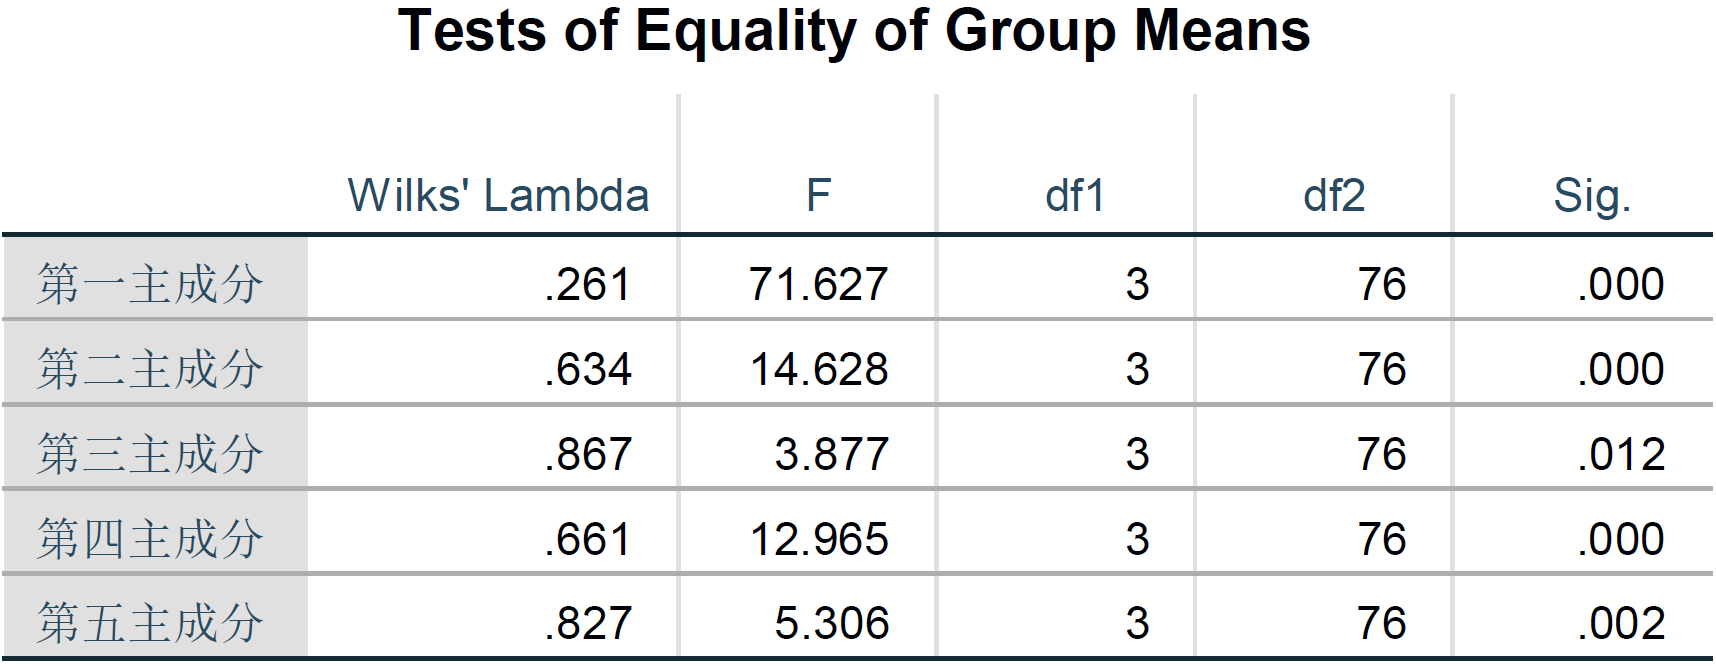
\includegraphics[scale=0.2]{主成分的均值检验.png}
    \end{center}
    \vspace{-0.5cm}
\end{frame}


\begin{frame}{对主成分协方差矩阵的 Box's M 检验}
    \begin{center}
        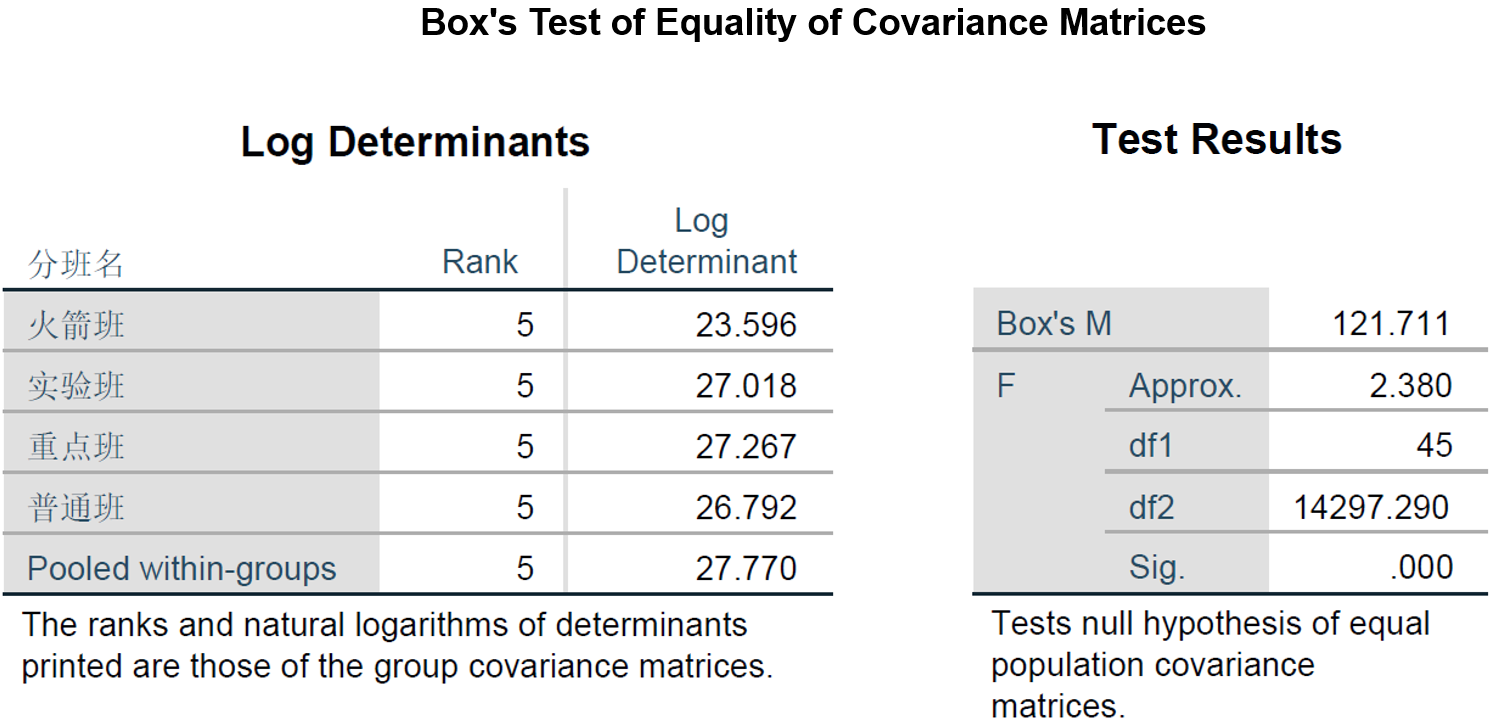
\includegraphics[scale=0.22]{协方差阵相等的检验.png}
    \end{center}
    \vspace{-0.5cm}
\end{frame}


\begin{frame}{Fisher 线性判别}
    \begin{center}
        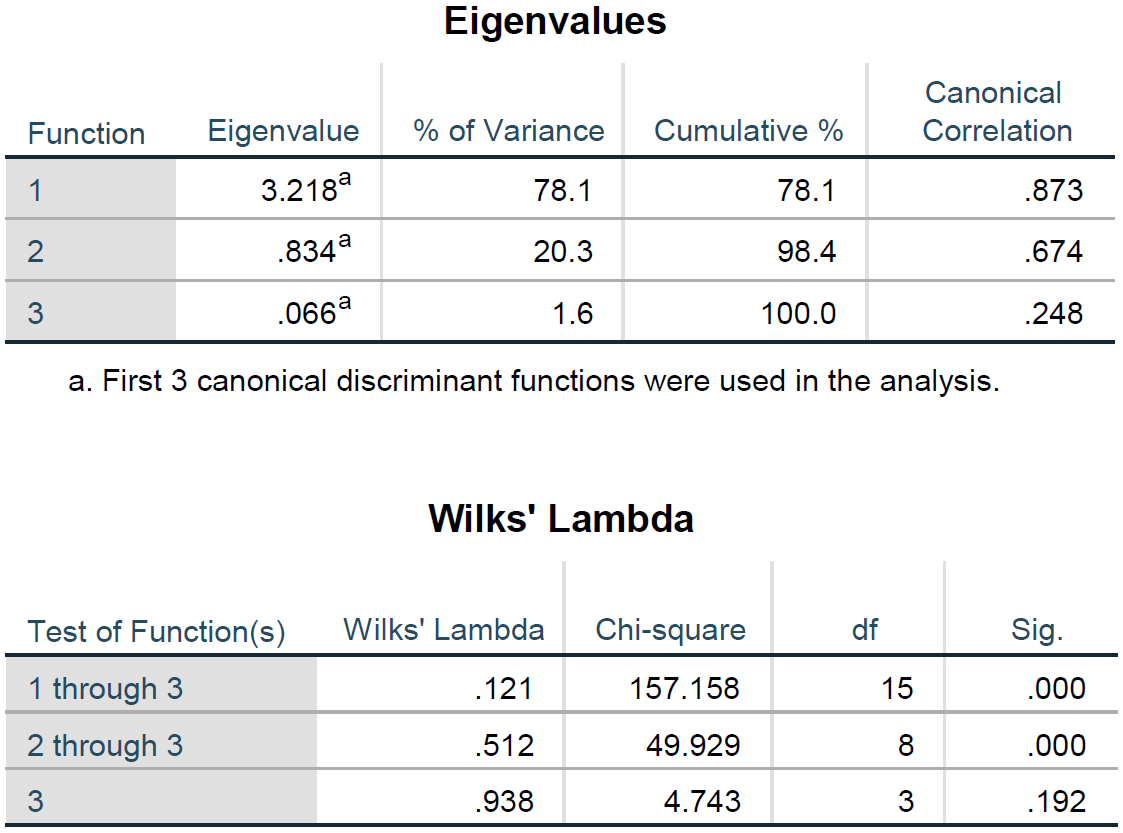
\includegraphics[scale=0.225]{判别函数特征根、解释方差比.png}
    \end{center}
    \vspace{-0.5cm}
\end{frame}


\begin{frame}{标准化/非标准化 Fisher 线性判别函数}

    \begin{center}
        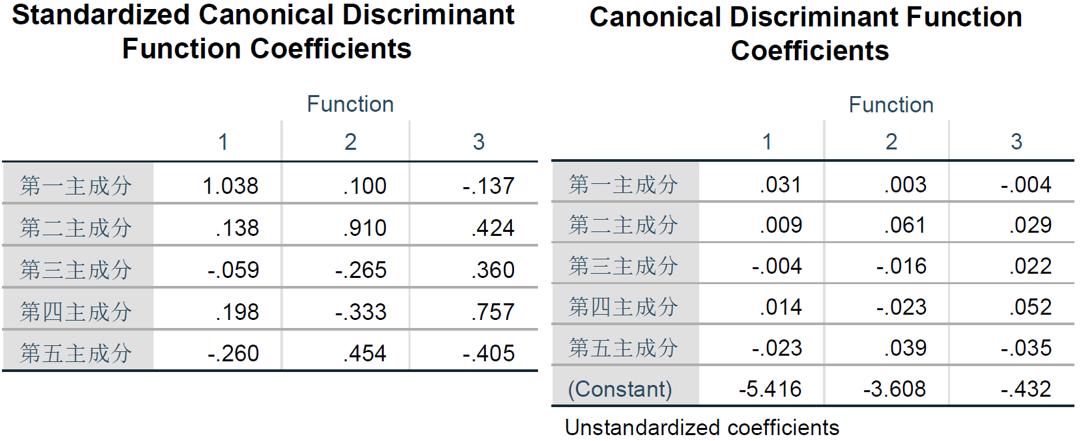
\includegraphics[scale=0.32]{标准化、非标准化判别系数.png}
    \end{center}
    \vspace{-0.5cm}

\end{frame}


% 分类函数.png
\begin{frame}{分类函数}
    \begin{center}
        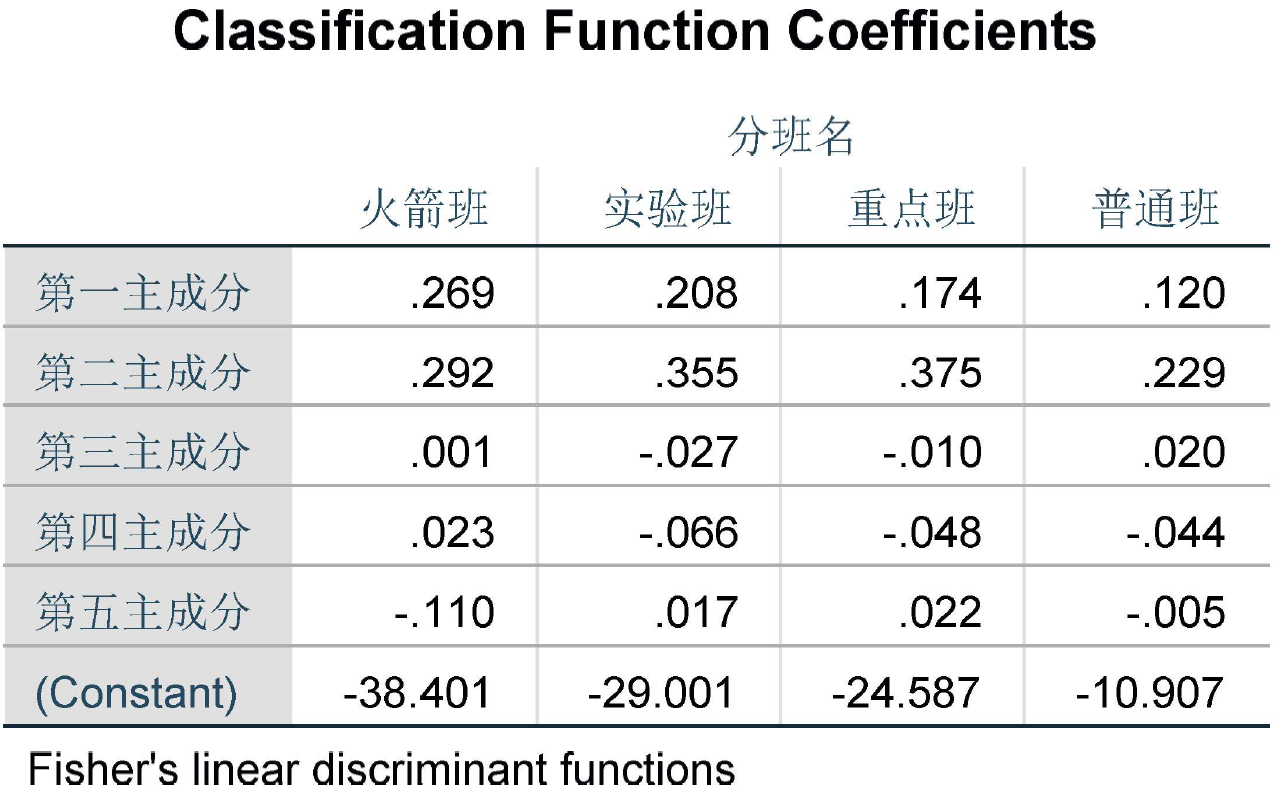
\includegraphics[scale=0.22]{分类函数.png}
    \end{center}
    \vspace{-0.5cm}
\end{frame}


% 分类结果.png
\begin{frame}{预测的分类结果}
    \begin{center}
        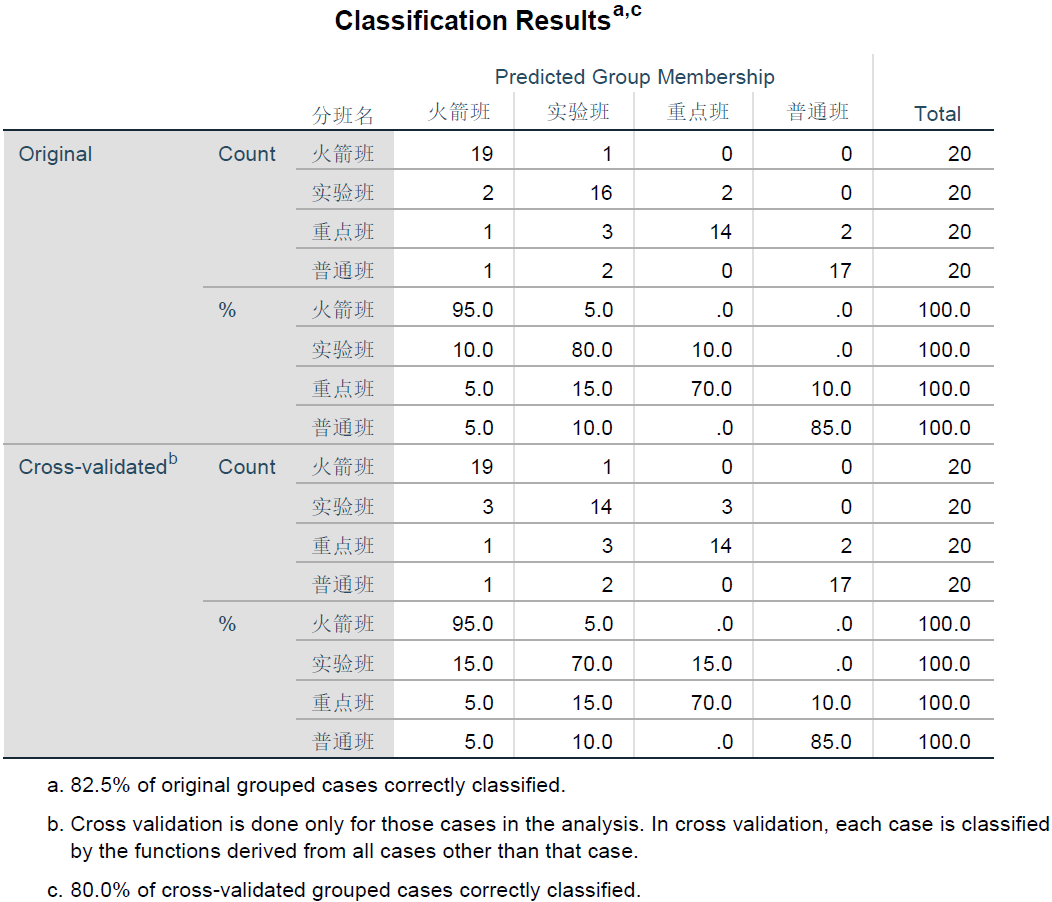
\includegraphics[scale=0.21]{分类结果.png}
    \end{center}
    \vspace{-0.5cm}
\end{frame}


% 分类结果图.png
\begin{frame}{预测的分类结果图}
    \begin{center}
        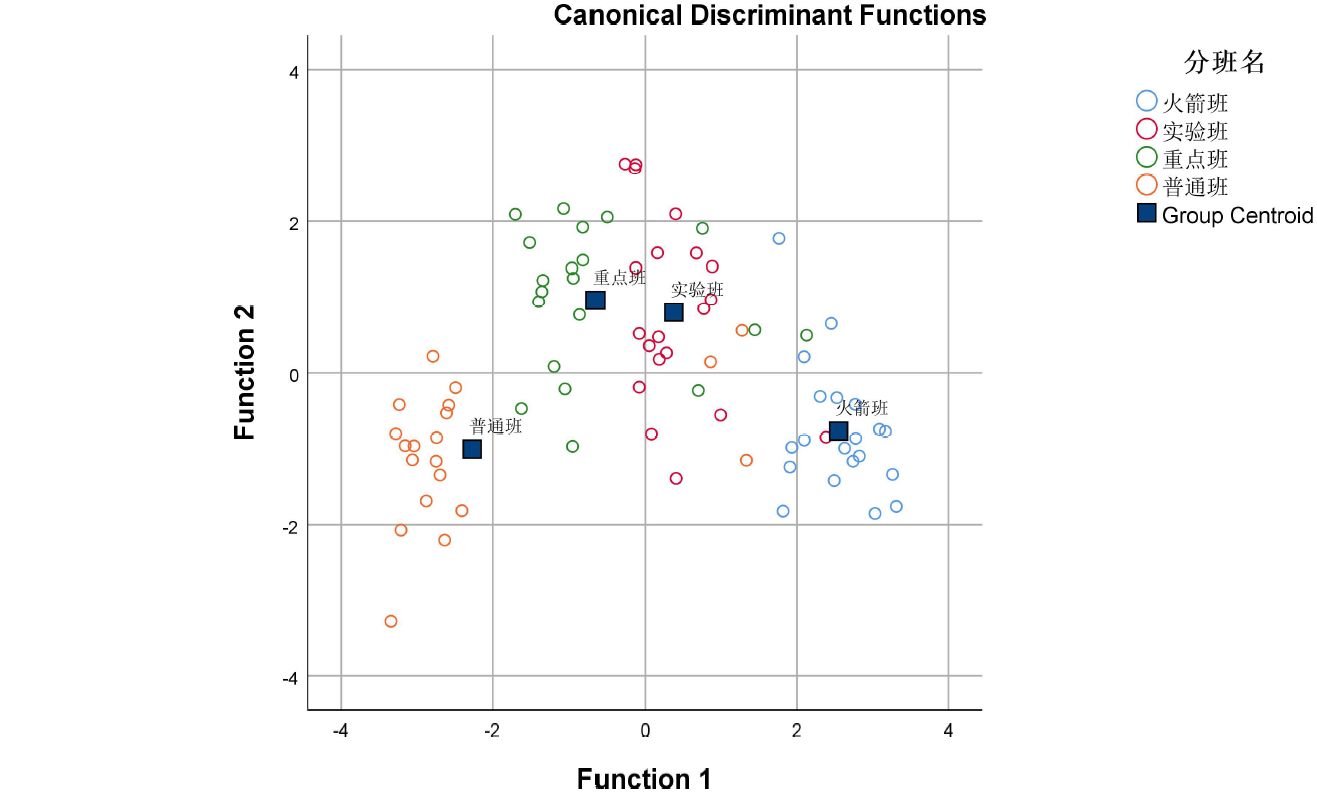
\includegraphics[scale=0.23]{分类结果图.png}
    \end{center}
    \vspace{-0.5cm}
\end{frame}
